\documentclass{standalone}
\usepackage{mathpazo}
\usepackage[american]{circuitikz}

\begin{document}
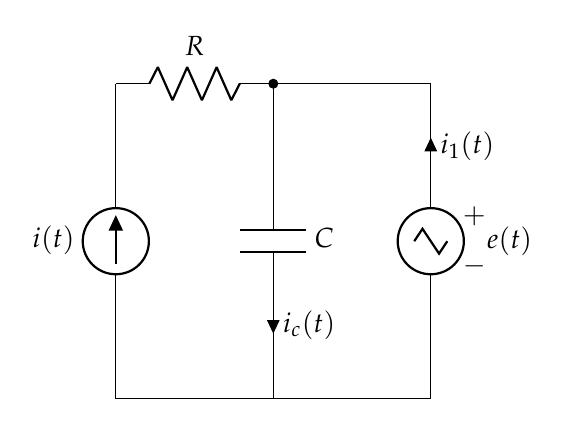
\begin{tikzpicture}
  \coordinate (A) at (0,4);
  \coordinate (B) at (2,4);
  \coordinate (C) at (4,4);
  \coordinate (D) at (0,0);
  \coordinate (E) at (2,0);
  \coordinate (F) at (4,0);
  \draw
  (A) to [R, l=$R$] (B)
  to [short] (C)
  to [tV, v = $e(t)$, i<= $i_1(t)$] (F)
  to [short] (D);
  \draw
  (D) to [isource, l=$i(t)$] (A);
  \draw
  (B) to [C, *-, l=$C$, i = $i_c(t)$] (E);
  \end{tikzpicture}
\end{document}